\phantomsection

% Increment the chapter counter so \thechapter shows the correct number
% and make it referenceable with \ref
\refstepcounter{chapter}

% Manually add this appendix to the Table of Contents
\addcontentsline{toc}{chapter}{Apéndice \thechapter: Configuración del universo Grid en la infraestructura HTCondor del Grupo GRID}

% Add vertical space above the title (mimics standard chapter spacing)
\vspace{40pt}

% Display the actual chapter title (centered, large, bold)
{\centering \normalfont\huge\bfseries Apéndice~\thechapter: Configuración del universo Grid en la infraestructura HTCondor del Grupo GRID~\par}

% Add spacing between title and horizontal rule
\vspace{10pt}

% Draw a horizontal line across the page for visual separation
{\centering \rule{\textwidth}{0.4pt} \par}

% Add vertical space between title section and content
\vspace{40pt}

% Set the running headers for left and right pages
\markboth{Apéndice \thechapter: Configuración del universo Grid}{Apéndice \thechapter: Configuración del universo Grid}

\FloatBarrier\subsection{Configuración del universo Grid}

El universo Grid de HTCondor permite la ejecución de trabajos a través de múltiples clústeres distribuidos geográficamente, facilitando el aprovechamiento de recursos computacionales heterogéneos. La infraestructura del Grupo \GRID implementa este universo mediante un nodo coordinador (\textit{grid manager}) que gestiona la distribución de trabajos hacia clústeres remotos con el universo Vanilla.

La configuración actual soporta la versión \texttt{8.4.11} de HTCondor en arquitectura \texttt{armv7l} sobre sistema operativo Raspbian GNU/Linux 9 (stretch). A continuación se muestra la salida del comando de versión en el nodo \textit{grid manager}:

% HTCondor version output
\begin{minted}[
    frame=lines,
    framesep=2mm,
    baselinestretch=1.2,
    bgcolor=lightgray!10,
    fontsize=\footnotesize,
]{bash}
$CondorVersion: 8.4.11 Feb 06 2017 BuildID: Debian-8.4.11~dfsg.1-1 Debian-8.4.11~dfsg.1-1 $
$CondorPlatform: ARMV7L-Raspbian_ $
\end{minted}

\FloatBarrier\subsubsection{Arquitectura del universo Grid}

El universo Grid en la infraestructura del Grupo~\GRID implementa una arquitectura federada donde un nodo coordinador central gestiona la distribución de trabajos hacia múltiples clústeres Vanilla independientes. Esta arquitectura permite la utilización de recursos distribuidos y proporciona tolerancia a fallos mediante la capacidad de redirigir trabajos entre diferentes clústeres.

\textbf{Componentes principales:}

\begin{itemize}
	\item \textbf{grid manager (172.30.27.11)}: Nodo coordinador que ejecuta los \textit{daemons} \texttt{SCHEDD}, \texttt{MASTER}, \texttt{GRIDMANAGER} y \texttt{COLLECTOR}, responsable de recibir trabajos desde la aplicación \textit{Grid App} y distribuirlos hacia los clústeres Vanilla disponibles.
	
	\item \textbf{Clúster Vanilla B}: Infraestructura computacional compuesta por un \textit{master/central manager} (172.30.27.34), un nodo \textit{submit} (172.30.27.35) y múltiples nodos \textit{Execute} (172.30.27.36-48).

	\item \textbf{Clúster Vanilla C}: Segunda infraestructura computacional con \textit{master/central manager} (172.30.27.66), nodo \textit{submit} (172.30.27.67) y nodos \textit{Execute} (172.30.27.68-80).
\end{itemize}

\begin{figure}
	\centering
	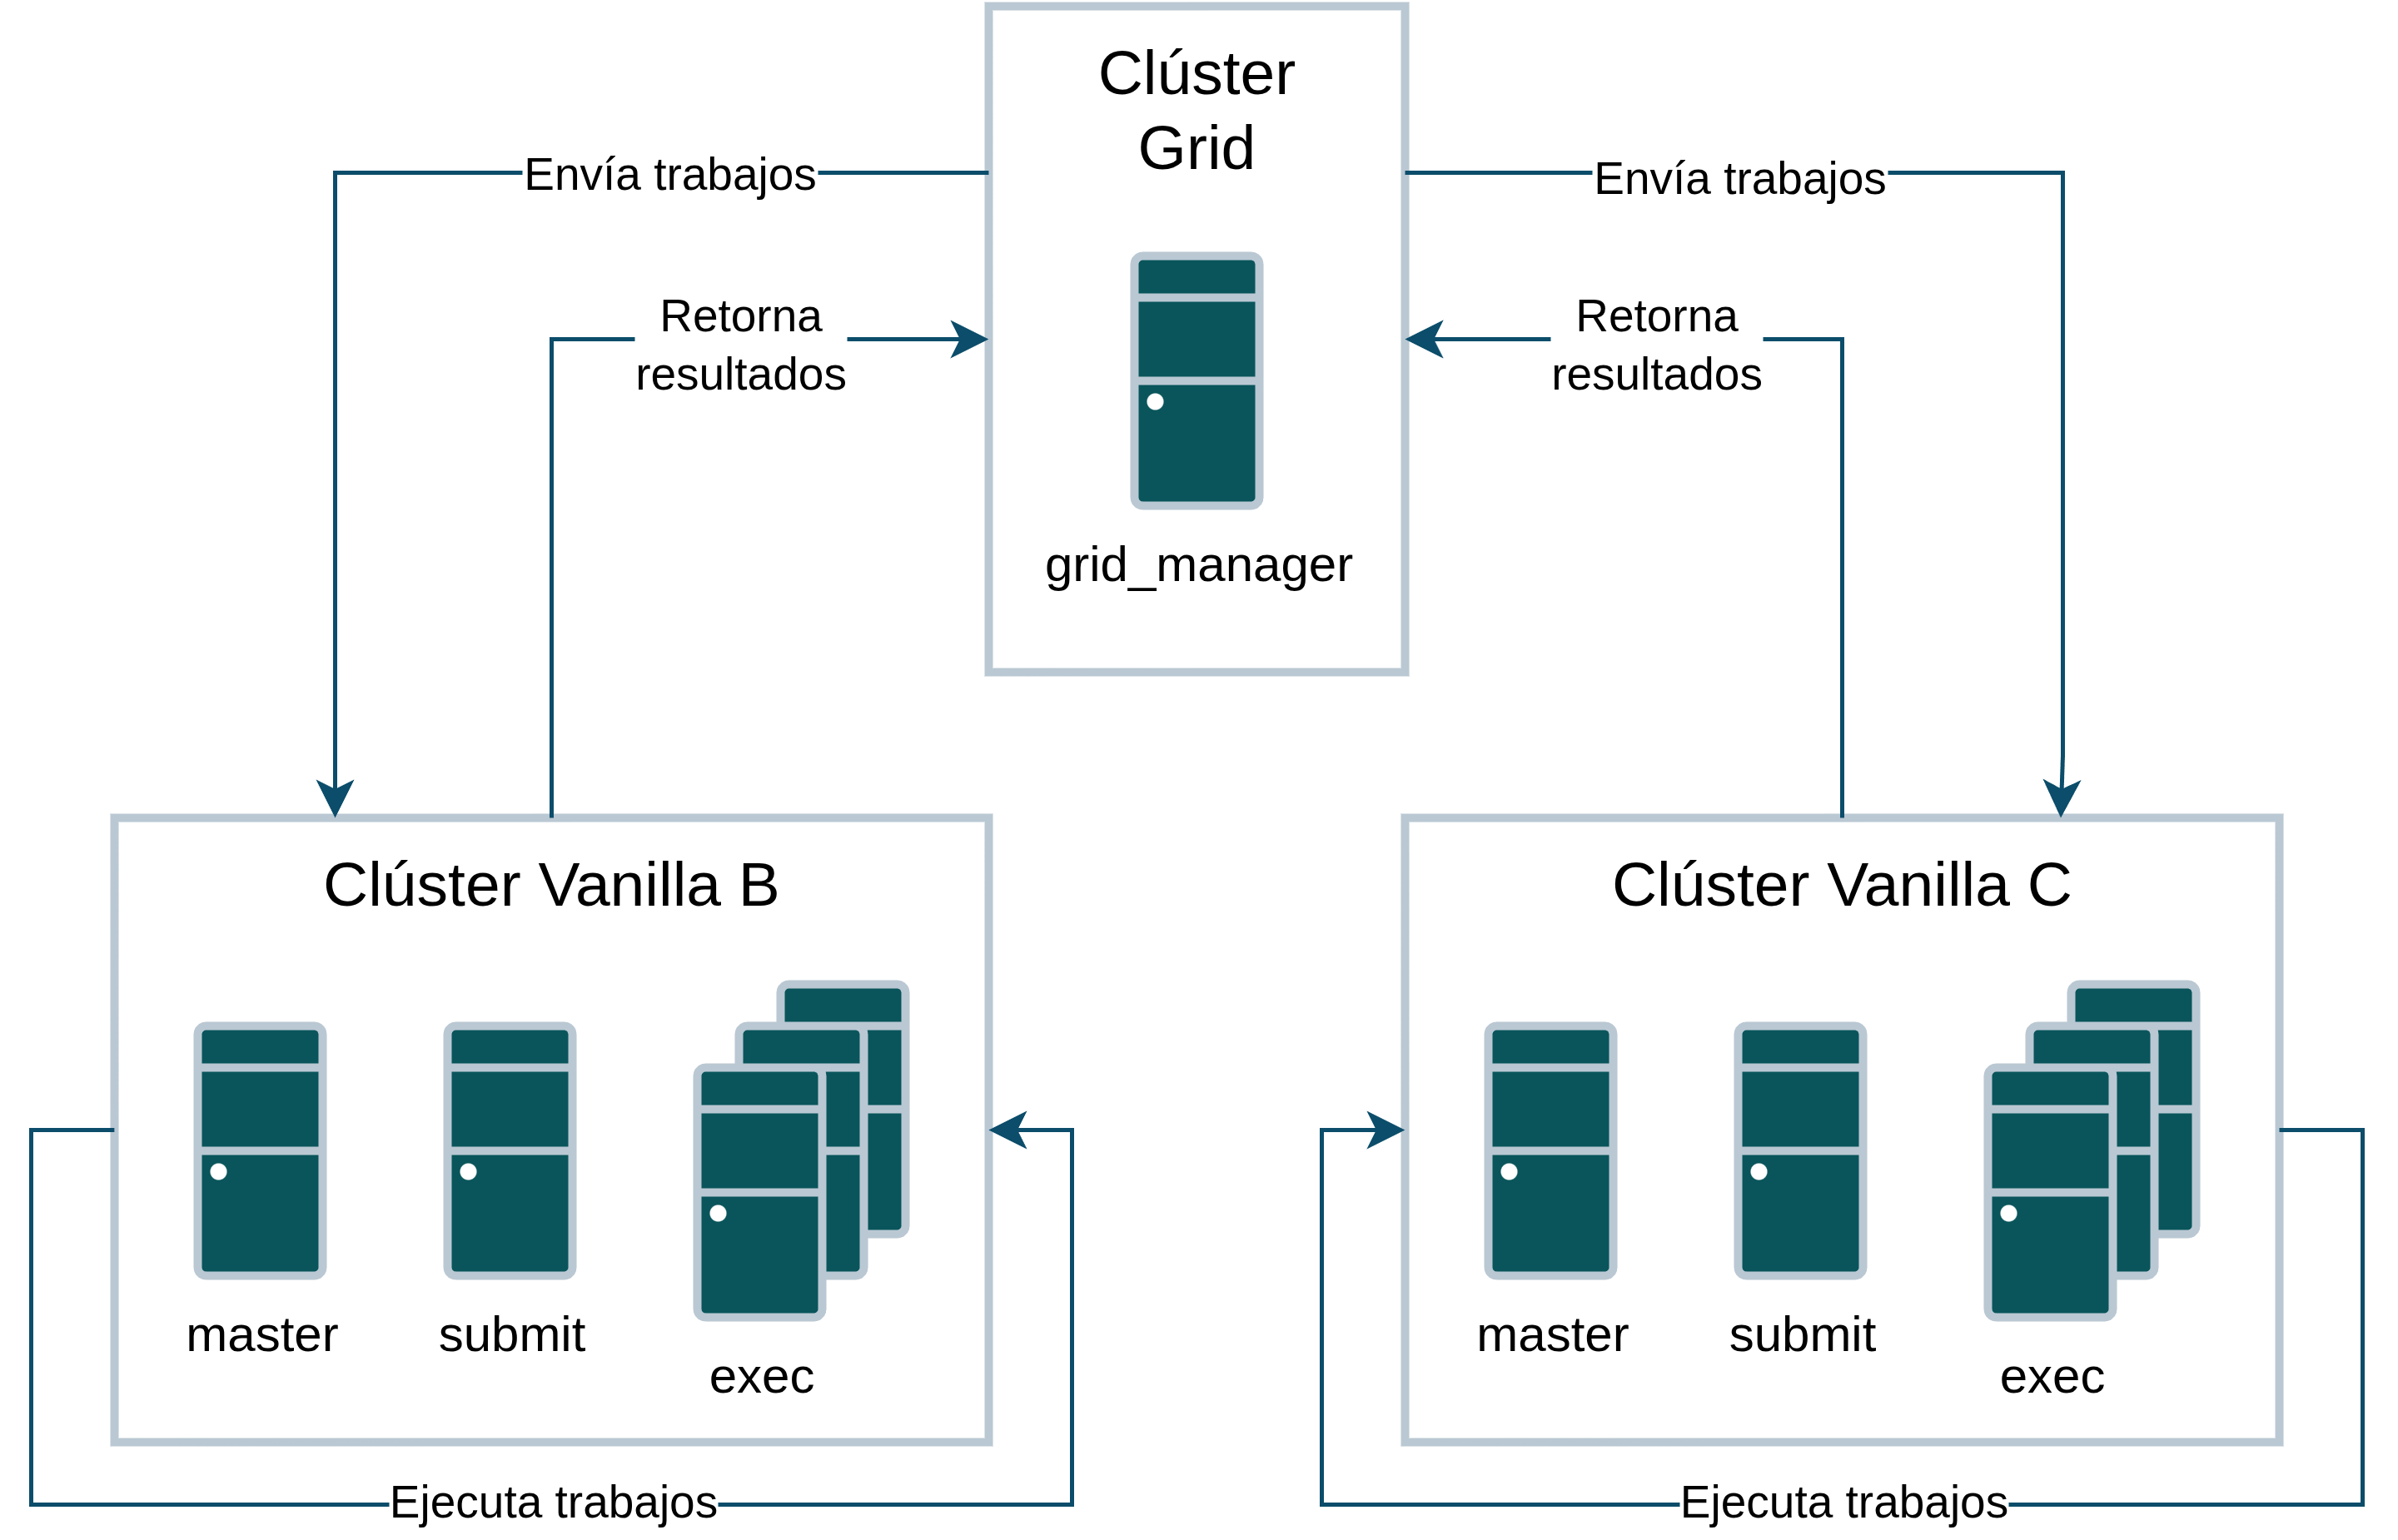
\includegraphics[scale=0.11]{apendices/infra-virtual/Diagramas HTCondor-Grid-flow.drawio.png}
	\caption{Arquitectura del universo Grid en la infraestructura HTCondor del~\GRID}
	\label{fig:grid-architecture}
\end{figure}

\FloatBarrier\subsubsection{Configuración del \textit{grid manager}}

El \textit{grid manager} constituye el componente central del universo Grid, implementando la lógica de distribución de trabajos y coordinación con clústeres remotos. Su configuración se basa en el archivo \texttt{/etc/condor/condor\_config.local} que define los parámetros específicos para su rol.

\textbf{Configuración de \textit{daemons}:}

La configuración especifica los \textit{daemons} que se ejecutan en el \textit{grid manager}:

\begin{minted}[
    frame=lines,
    framesep=2mm,
    baselinestretch=1.2,
    bgcolor=lightgray!10,
    fontsize=\footnotesize,
]{bash}
# Daemons ejecutados en el grid manager
DAEMON_LIST = SCHEDD, MASTER, GRIDMANAGER, COLLECTOR
\end{minted}

\textbf{Configuración específica del universo Grid:}

\begin{minted}[
    frame=lines,
    framesep=2mm,
    baselinestretch=1.2,
    bgcolor=lightgray!10,
    fontsize=\footnotesize,
]{bash}
# Variables específicas para el universo Grid
CONDOR_GAHP = $(SBIN)/condor_c-gahp
C_GAHP_LOG = /tmp/CGAHPLog.$(USERNAME)
C_GAHP_WORKER_THREAD_LOG = /tmp/CGAHPWorkerLog.$(USERNAME)
C_GAHP_WORKER_THREAD_LOCK = /tmp/CGAHPWorkerLock.$(USERNAME)
\end{minted}

\textbf{Configuración de seguridad:}

La configuración de seguridad implementa autenticación opcional para facilitar la comunicación entre nodos en una red confiable:

\begin{minted}[
    frame=lines,
    framesep=2mm,
    baselinestretch=1.2,
    bgcolor=lightgray!10,
    fontsize=\footnotesize,
]{bash}
# Configuración de seguridad minima para cluster en red confiable
SEC_DEFAULT_AUTHENTICATION = OPTIONAL
SEC_DEFAULT_AUTHENTICATION_METHODS = CLAIMTOBE,FS
SEC_DEFAULT_ENCRYPTION = OPTIONAL
SEC_DEFAULT_INTEGRITY = OPTIONAL
\end{minted}

\textbf{Permisos de acceso:}

\begin{minted}[
    frame=lines,
    framesep=2mm,
    baselinestretch=1.2,
    bgcolor=lightgray!10,
    fontsize=\footnotesize,
]{bash}
# Permisos para el daemon SCHEDD
ALLOW_READ_SCHEDD = 172.30.27.43, 127.0.0.1, rb3-*
ALLOW_WRITE_SCHEDD = 172.30.27.43, 127.0.0.1, rb3-*

# Permisos generales de red
ALLOW_READ  = 172.30.*
ALLOW_WRITE = 172.30.*
\end{minted}

\textbf{Configuración de red:}

\begin{minted}[
    frame=lines,
    framesep=2mm,
    baselinestretch=1.2,
    bgcolor=lightgray!10,
    fontsize=\footnotesize,
]{bash}
# Configuración de interfaz de red específica
BIND_ALL_INTERFACES = FALSE
NETWORK_INTERFACE = 172.30.27.11

# Configuración de dominio
FILESYSTEM_DOMAIN = $(FULL_HOSTNAME)
UID_DOMAIN = uniquindio.edu.co
CONDOR_HOST = rb3-t01-1
\end{minted}

\FloatBarrier\subsection{Configuración de clústeres Vanilla}

Los clústeres Vanilla constituyen los recursos computacionales donde se ejecutan finalmente los trabajos distribuidos desde el clúster Grid. La configuración de estos clústeres fue adaptada durante este proyecto para habilitar la recepción y ejecución de trabajos provenientes del universo Grid.

\FloatBarrier\subsubsection{Configuración del nodo \textit{submit}}

El nodo \textit{submit} de cada clúster Vanilla actúa como punto de entrada para trabajos provenientes del \textit{grid manager}. Su configuración habilita tanto funcionalidades locales como la capacidad de recibir trabajos remotos.

\textbf{Configuración de \textit{daemons}:}

\begin{minted}[
    frame=lines,
    framesep=2mm,
    baselinestretch=1.2,
    bgcolor=lightgray!10,
    fontsize=\footnotesize,
]{bash}
# Daemons ejecutados en el nodo submit
DAEMON_LIST = SCHEDD, MASTER
\end{minted}

\textbf{Habilitación del universo Grid:}

\begin{minted}[
    frame=lines,
    framesep=2mm,
    baselinestretch=1.2,
    bgcolor=lightgray!10,
    fontsize=\footnotesize,
]{bash}
# Habilitación explícita del universo Grid
ENABLE_GRID_UNIVERSE = True

# Configuración específica para SCHEDD
SCHEDD_ADDRESS_FILE = $(LOG)/.schedd_address
BIND_ALL_INTERFACES = FALSE
\end{minted}

\textbf{Permisos para grid manager:}

\begin{minted}[
    frame=lines,
    framesep=2mm,
    baselinestretch=1.2,
    bgcolor=lightgray!10,
    fontsize=\footnotesize,
]{bash}
# Permisos específicos para grid manager
ALLOW_WRITE_SCHEDD = 172.30.27.43, 127.0.0.1
ALLOW_READ_SCHEDD = 172.30.27.43, 127.0.0.1
HOSTALLOW_WRITE = 172.30.27.43, 127.0.0.1
\end{minted}

\textbf{Configuración de usuarios y autenticación:}

Una configuración crítica para el funcionamiento del universo Grid es la gestión de usuarios y autenticación entre nodos:

\begin{minted}[
    frame=lines,
    framesep=2mm,
    baselinestretch=1.2,
    bgcolor=lightgray!10,
    fontsize=\footnotesize,
]{bash}
# Usuarios con privilegios especiales
QUEUE_SUPER_USERS = root, condor, CONDOR_ANONYMOUS_USER, alma
UID_DOMAIN = gridmanager

# Habilitación de usuarios anónimos
ALLOW_WRITE = *, anonymous@*
ALLOW_READ = *, anonymous@*
ALLOW_ADMINISTRATOR = *, $(FULL_HOSTNAME), $(IP_ADDRESS)
ALLOW_OWNER = *

# Usuario anónimo para condor
CONDOR_ANONYMOUS_USER = nobody

# Configuración de autenticación
SEC_READ_AUTHENTICATION = OPTIONAL
SEC_WRITE_AUTHENTICATION = OPTIONAL
SEC_ADMINISTRATOR_AUTHENTICATION = OPTIONAL

SCHEDD.ALLOW_ANONYMOUS_USER = TRUE
\end{minted}

\FloatBarrier\subsubsection{Configuración del nodo \textit{master/central manager}}

El nodo \textit{master/central manager} de cada clúster Vanilla coordina los recursos locales y facilita la comunicación con el \textit{grid manager}:

\textbf{Configuración de \textit{daemons}:}

\begin{minted}[
    frame=lines,
    framesep=2mm,
    baselinestretch=1.2,
    bgcolor=lightgray!10,
    fontsize=\footnotesize,
]{bash}
# Daemons ejecutados en el central manager
DAEMON_LIST = COLLECTOR, NEGOTIATOR, MASTER
\end{minted}

\textbf{Configuración de red y permisos:}

\begin{minted}[
    frame=lines,
    framesep=2mm,
    baselinestretch=1.2,
    bgcolor=lightgray!10,
    fontsize=\footnotesize,
]{bash}
# Configuración de red específica para Clúster B
NETWORK_INTERFACE = 172.30.27.34  # Para central manager del Clúster B
# NETWORK_INTERFACE = 172.30.27.66  # Para central manager del Clúster C

# Nodo coordinador del clúster
CONDOR_HOST = rb3-t06-1  # Para Clúster B
# CONDOR_HOST = rb3-t06-4  # Para Clúster C

# Permisos de red amplios para comunicación Grid
ALLOW_READ  = 172.30.*
ALLOW_WRITE = 172.30.*
\end{minted}

\FloatBarrier\subsubsection{Configuración de nodos \textit{Execute}}

Los nodos \textit{Execute} proporcionan los recursos computacionales donde se ejecutan los trabajos. Su configuración permite recibir trabajos tanto locales como provenientes del \textit{grid manager}:

\textbf{Configuración de \textit{daemons}:}

\begin{minted}[
    frame=lines,
    framesep=2mm,
    baselinestretch=1.2,
    bgcolor=lightgray!10,
    fontsize=\footnotesize,
]{bash}
# Daemons ejecutados en nodos Execute
DAEMON_LIST = STARTD, MASTER
\end{minted}

\FloatBarrier\subsection{Configuración de red y resolución de nombres}

Una configuración crítica para el funcionamiento del universo Grid es la resolución de nombres entre todos los nodos participantes. El archivo \texttt{/etc/hosts} en cada nodo debe contener las entradas correspondientes a todos los nodos de la infraestructura.

\textbf{Configuración completa del archivo \texttt{/etc/hosts}:}

\begin{minted}[
    frame=lines,
    framesep=2mm,
    baselinestretch=1.2,
    bgcolor=lightgray!10,
    fontsize=\footnotesize,
]{bash}
127.0.0.1       localhost

# grid manager
172.30.27.11    rb3-t01-1

# Clúster B - Vanilla
# master
172.30.27.34    rb3-t06-1
# submit
172.30.27.35    rb3-t06-2
# Execute nodes
172.30.27.36    rb3-t02-1
172.30.27.37    rb3-t02-2
172.30.27.38    rb3-t02-3
172.30.27.39    rb3-t02-4
172.30.27.40    rb3-t02-5
172.30.27.41    rb3-t02-6
172.30.27.42    rb3-t02-7
172.30.27.43    rb3-t03-2
172.30.27.44    rb3-t03-3
172.30.27.45    rb3-t03-4
172.30.27.46    rb3-t03-5
172.30.27.47    rb3-t03-6
172.30.27.48    rb3-t03-7

# Clúster C - Vanilla
# master
172.30.27.66    rb3-t06-4
# submit
172.30.27.67    rb3-t06-5
# Execute nodes
172.30.27.68    rb3-t04-1
172.30.27.69    rb3-t04-2
172.30.27.70    rb3-t04-3
172.30.27.71    rb3-t04-4
172.30.27.72    rb3-t04-6
172.30.27.73    rb3-t04-7
172.30.27.74    rb3-t05-1
172.30.27.75    rb3-t05-2
172.30.27.76    rb3-t05-3
172.30.27.77    rb3-t05-4
172.30.27.78    rb3-t05-5
172.30.27.79    rb3-t05-6
172.30.27.80    rb3-t05-7
\end{minted}

\FloatBarrier\subsection{Expansión de la infraestructura Vanilla}

Durante el desarrollo de este proyecto se realizó la expansión de la infraestructura Vanilla existente, pasando de un único clúster a dos clústeres independientes (Clúster B y Clúster C). Esta expansión fue necesaria para demostrar la capacidad de distribución de trabajos del universo Grid y proporcionar redundancia en la infraestructura.

\textbf{Beneficios de la expansión:}

\begin{itemize}
	\item \textbf{Mayor capacidad computacional}: Duplicación de los recursos disponibles para ejecución de trabajos.
	
	\item \textbf{Redundancia}: Capacidad de continuar operaciones en caso de falla de un clúster completo.
	
	\item \textbf{Balanceo de carga}: Distribución automática de trabajos según disponibilidad de recursos.
	
	\item \textbf{Escalabilidad}: Demostración de que la arquitectura puede expandirse a múltiples clústeres adicionales.
\end{itemize}

\FloatBarrier\subsection{Verificación de la configuración}

Una vez completada la configuración, es posible verificar el correcto funcionamiento del universo Grid mediante varios comandos de diagnóstico:

\textbf{Verificación desde el universo Grid:}

\begin{minted}[
    frame=lines,
    framesep=2mm,
    baselinestretch=1.2,
    bgcolor=lightgray!10,
    fontsize=\footnotesize,
]{bash}
# Verificar conectividad con clústeres remotos
condor_status -pool rb3-t06-1

# Verificar configuración local del SCHEDD
condor_config_val -schedd DAEMON_LIST

# Verificar logs del grid manager
tail -f /var/log/condor/GridmanagerLog
\end{minted}

\textbf{Verificación desde clústeres Vanilla:}

\begin{minted}[
    frame=lines,
    framesep=2mm,
    baselinestretch=1.2,
    bgcolor=lightgray!10,
    fontsize=\footnotesize,
]{bash}
# Verificar disponibilidad de recursos
condor_status

# Verificar permisos de grid manager
condor_config_val ALLOW_WRITE_SCHEDD
\end{minted}

\FloatBarrier\subsection{Consideraciones importantes}

\textbf{Limitaciones del alcance:}

Es importante destacar que este proyecto se enfocó específicamente en la adaptación de la infraestructura Vanilla existente para soportar trabajos provenientes del universo Grid. La instalación inicial de HTCondor en los dispositivos Raspberry Pi fue realizada previamente y no formó parte del alcance de este trabajo.

\textbf{Configuración específica del entorno:}

Las configuraciones presentadas están diseñadas para el entorno específico del Grupo \GRID, incluyendo:

\begin{itemize}
	\item Arquitectura ARM de 32 bits (armv7l)
	\item Sistema operativo Raspbian GNU/Linux 9 (stretch)
	\item HTCondor versión 8.4.11
	\item Red interna confiable (172.30.27.0/24)
\end{itemize}

\textbf{Escalabilidad de la solución:}

La configuración implementada permite la adición de clústeres Vanilla adicionales mediante la replicación de la configuración base y la actualización de las tablas de enrutamiento de red. Esta característica facilita el crecimiento futuro de la infraestructura según las necesidades computacionales del grupo de investigación.

\textbf{Seguridad y confiabilidad:}

La configuración de seguridad mínima (autenticación opcional) está justificada por el entorno de red confiable y controlado donde opera la infraestructura. En entornos de producción o redes menos confiables, sería necesario implementar políticas de seguridad más estrictas, incluyendo autenticación obligatoria y cifrado de comunicaciones.
